\documentclass[spanish]{beamer}
\usepackage[ansinew]{inputenc} % Acepta caracteres en castellano
\usepackage[spanish]{babel}    % silabea palabras castellanas
\usepackage{amsmath}
\usepackage{amsfonts}
\usepackage{amssymb}
\usepackage{dsfont}
\usepackage{graphicx}
\usepackage{geometry}
\usetheme{Madrid}
\usecolortheme{beaver}
\usepackage{textpos}
% Logo  en el comienzo 
\addtobeamertemplate{frametitle}{}{%
\begin{textblock*}{100mm}(.85\textwidth,-1cm)
{\includegraphics[height=0.4in, keepaspectratio=true]{/Users/luisnunez/Dropbox/MisDocumentos/UIS/UISImagenInstitucional/UISLOGO.png}}
\end{textblock*}}

\begin{document}

\title{\textbf{Braquistocrona} }
\author[L.A. N��ez]{\textbf{Luis A. N��ez}}  
\institute[UIS]{\textit{Escuela de F�sica, Facultad de Ciencias, } \\
\textit{Universidad Industrial de Santander, Santander, Colombia } \\
{\includegraphics[height=0.4in, keepaspectratio=true]{/Users/luisnunez/Dropbox/MisDocumentos/UIS/UISImagenInstitucional/UISLOGO.png}}
}
\date{\today}
\maketitle


\begin{frame}
\frametitle{Agenda}
  \tableofcontents
\end{frame}


%%%%% Diapo 1
\section{El problema}
\frame{
  \frametitle{El Problema}
   \begin{itemize}  
  	\item<1-> Encontrar la trayectoria $y(x)$ de una part�cula, que en un movimiento sin fricci�n, partiendo del reposo y sometida a un campo gravitatorio terrestre, que emplea el menor tiempo para ir de un punto $(x_1, y_1)$ a otro punto $(x_2, y_2)$.
  	\begin{figure}[t]
		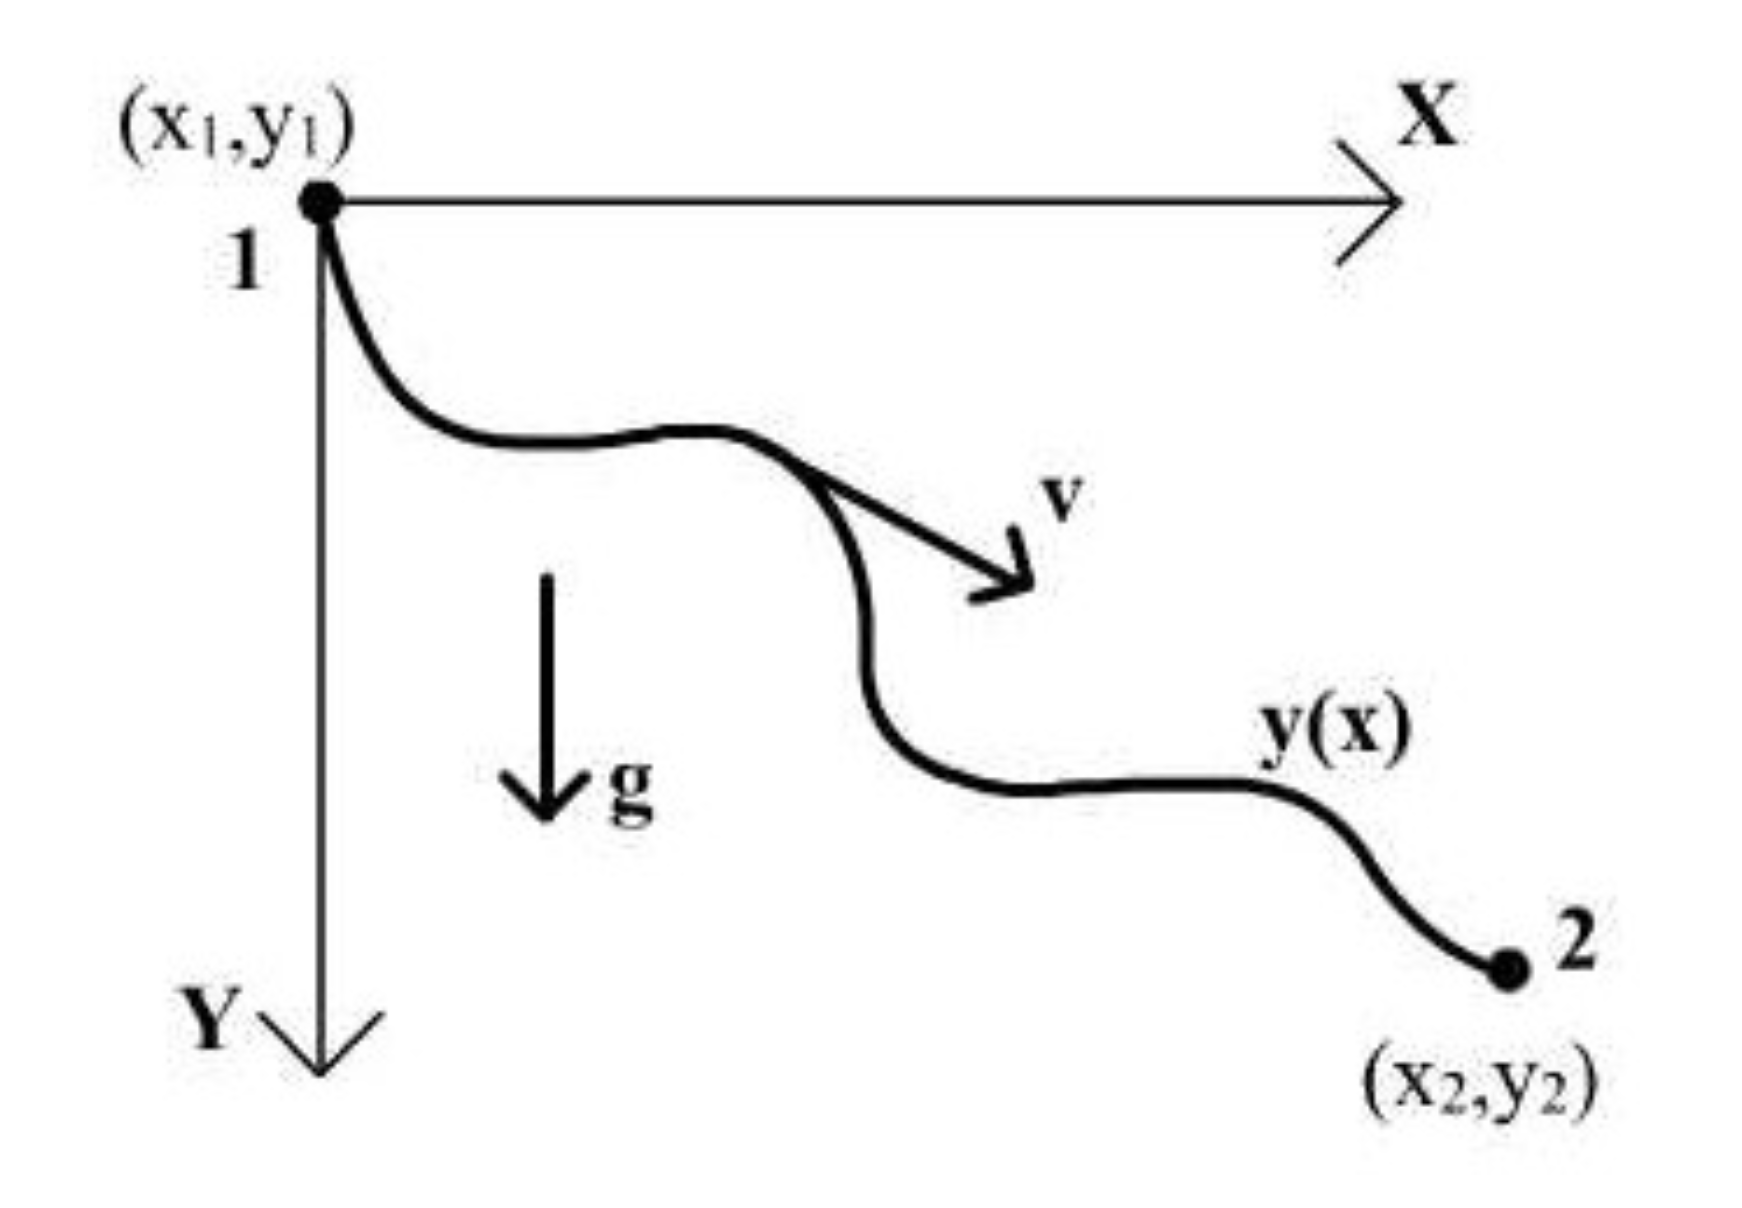
\includegraphics[width=2.4in]{Figuras/Braquistocrona.png} 
	\end{figure}  
    \end{itemize}
}
%%%%% Diapo 2
\section{El funcional y la Ecuaci�n Euler}
\frame{
  \frametitle{El funcional y la ecuaci�n de Euler}
   \begin{itemize}  
  	\item<1->  Fijamos el punto $(x_1, y_1) = (0,0)$ y la direcci�n del eje $y$ hacia abajo.
	\item<2->  Si $v$ es la magnitud de la velocidad en un punto de la trayectoria, entonces el elemento de tiempo para recorrer una distancia infinitesimal ${\rm d}s$ a lo largo de la trayectoria es $d t=\frac{{\rm d} s}{v}$.
	\item<3-> El tiempo total para ir del punto 1 al punto 2 es $t_{1 \rightarrow 2}=\int_1^2 \frac{{\rm d} s}{v}=\int_1^2 \frac{\sqrt{{\rm d} x^2 +{\rm d} y^2}}{v} =\int_{y_1}^{y_2} \sqrt{\frac{1+\left(x^{\prime}\right)^2}{2 g y}} {\rm d} y $
	\item<4-> Identificamos el funci�n del funcional $f\left(x, x^{\prime}, y\right)=\sqrt{\frac{1+\left(x^{\prime}\right)^2}{2 g y}}$
	\item<5-> La ecuaci�n de Euler correspondiente es $\frac{{\rm d}}{{\rm d} y}\left(\frac{\partial f}{\partial x^{\prime}}\right)-\frac{\partial f}{\partial x}= 0 \Rightarrow \frac{x^{\prime}}{\sqrt{2 g y} \sqrt{1+\left(x^{\prime}\right)^2}}=c=$ constante
	\item<6-> En este caso la ecuaci�n de Euler para  $f\left(x, x^{\prime}, y\right)$ resulta m�s sencilla que para $f\left(y, y^{\prime}, x\right)$, porque $\frac{\partial f}{\partial x}=0$
	\item<7-> Entonces $x^{\prime}  =\frac{{\rm d} x}{{\rm d} y}=\sqrt{\frac{2 g c^2 y}{1-2 g c^2 y}} \Rightarrow x  =\int \sqrt{\frac{y}{\frac{1}{2 g c^2}-y}} {\rm d} y=\int \sqrt{\frac{y}{2 R-y}} {\rm d} y, $ con $2 R \equiv 1 / 2 g c^2$
    \end{itemize}
}

%%%%% Diapo 2
\section{La trayectoria}
\frame{
  \frametitle{La trayectoria}
  \begin{itemize}  
  	\item<1-> Con un cambio de variable $y=R(1-\cos \theta), \quad {\rm d} y=R {\rm sen}\, \theta {\rm d} \theta$, tendremos $x  =R \int \sqrt{\frac{(1-\cos \theta)}{(1+\cos \theta)}} {\rm sen}\, \theta \;  {\rm d} \theta = R \int(1-\cos \theta) {\rm d} \theta $
	\item<2-> La trayectoria queda parametrizada por \\ $y=R(1-\cos \theta)$ y $x=R(\theta-{\rm sen}\, \theta)$. \\ La ecuaci�n de la cicloide que pasa por $\left(x_1, y_1\right)=(0,0)$, con $k=0$.
	\item<3-> La constante $R$ se determina con el punto $\left(x_2, y_2\right)$ y da al valor del radio de la circunferencia que genera la cicloide.
	\item<4-> La trayectoria de tiempo m�nimo es un arco de cicloide que pasa por los puntos dados $\theta_{\frac{\pi}{2}}  \Rightarrow y=R, x=\frac{\pi}{2} R$, $\theta_{\pi} \Rightarrow x=\pi R, y=2 R$ y $\theta_{2 \pi} \Rightarrow x=2 \pi R, y=0$
  	\begin{figure}[t]
		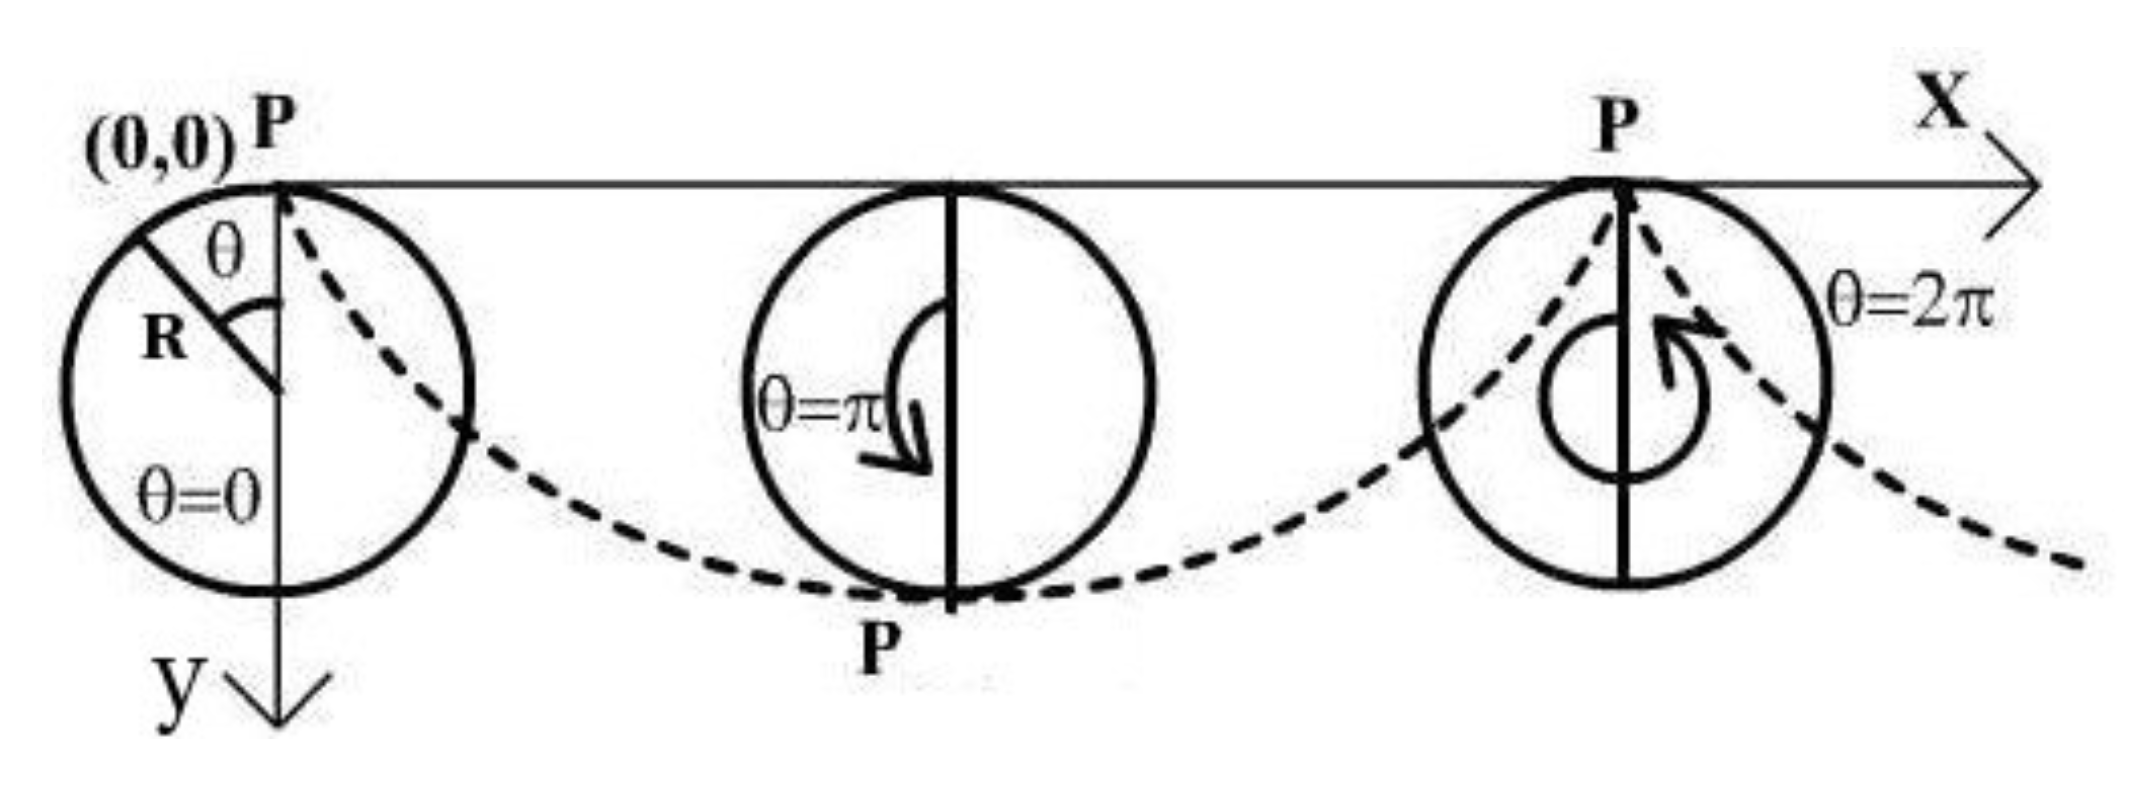
\includegraphics[width=2.4in]{Figuras/Cicloide.png} 
	\end{figure}  

   \end{itemize}
}

  
\end{document}

%%%%% Diapo 2
\section{Secci�n}
\frame{
  \frametitle{T�tulo transparencia}
  \begin{itemize}  
  	\item<1-> 
   \end{itemize}
}
%%%%% Diapo 2
\section{Secci�n}
\frame{
  \frametitle{T�tulo transparencia}
  \begin{itemize}  
  	\item<1-> 
   \end{itemize}
}
%%%%% Diapo 2
\section{Secci�n}
\frame{
  \frametitle{T�tulo transparencia}
  \begin{itemize}  
  	\item<1-> 
   \end{itemize}
}
%%%%% Diapo 2
\section{Secci�n}
\frame{
  \frametitle{T�tulo transparencia}
  \begin{itemize}  
  	\item<1-> 
   \end{itemize}
}

